
\subsection{Effects of Stabilization Policies}
We now analyze how the effects of energy price shocks can be influenced by policy measures as described in section \ref{92_energy}.
We consider the worst case scenario of a prolonged energy crisis with $12$ cumulative shocks of $5\%$ ($d=240$, $\pi=0.05$, $\Pi=20$).
Figure \ref{Figure: energy shock 4 growth} shows the GDP growth rate during the energy crisis of the previous section. 

As discussed in section \ref{92_energy}, we need to set the trigger for the policy.
The first trigger we set to $-5\%$, which means that the subsidy will not take effect until the annualized growth rate of GDP falls below $-5\%$. Note that the government in our model only detects this trigger once a year, so it really has to be a sustained economic downturn before the policy takes effect. In the example the subsidy would be activated around iteration 1200, when the economy first reaches below $-5\%$ growth.

The second trigger is set the $+5\%$ which in our example means that the subsidy would only be turned off at iteration 1600, when the economy starts to grow by more than $+5\%$ on a yearly basis. After that it never reaches below $-5\%$ again so the subsidy will remain inactive.

Figure \ref{Figure: Stabilization} shows the effect of the stabilizing subsidy. 
There is still the sharp downturn of $-15\%$ at period $1500$ following the energy crisis -- which lasts from periods $1240-1480$ -- but after the subsidy regime the growth rate is back to positive levels of $10\%$ to $30\%$, which is financed by the government subsidy. The subsidy is actually already activated before the energy crisis hits at period $1240$, but it grows in intensity as the crisis worsens, and gets switched of as soon as the growth rate reaches $+5\%$ again. Note however that the government does not register this until the end of the calendar year at period $1680$, so it has a lagged response in switching off the subsidy. On the longer term the GDP growth is between $0$ and $20\%$ instead of the previous levels of $0$ and $5\%$. The right panel in the figure shows that the subsidy gets re-activated three times more, whenever the growth drops below the trigger of $5\%$.

\begin{figure}[ht!]
\centering\leavevmode
\begin{minipage}{17cm}
\centering\leavevmode
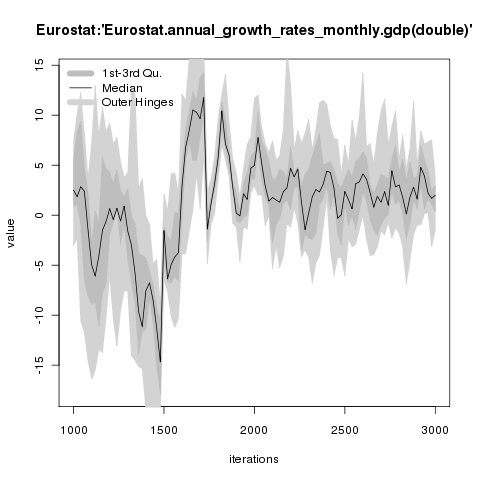
\includegraphics[width=8cm]{./energy_shock/png/duration_240/intensity_0.05/frequency_20/Eurostat-annual_growth_rates_monthly_gdp.png}
\end{minipage}
\caption{Growth rate of GDP during the energy crisis.}
\label{Figure: energy shock 4 growth}
\end{figure}

\begin{figure}[ht!]
\centering\leavevmode
\begin{minipage}{17cm}
\centering\leavevmode
%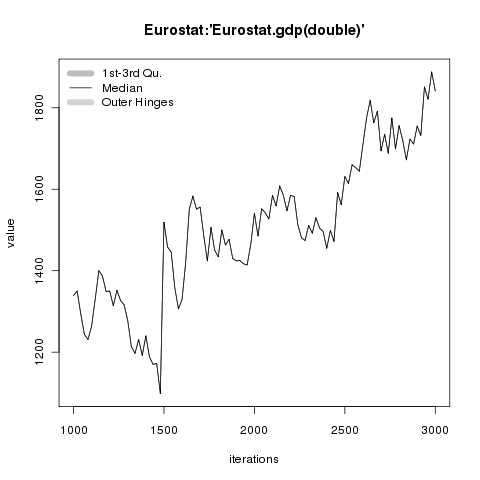
\includegraphics[width=8cm]{./stabilization/png/Eurostat-gdp.png}
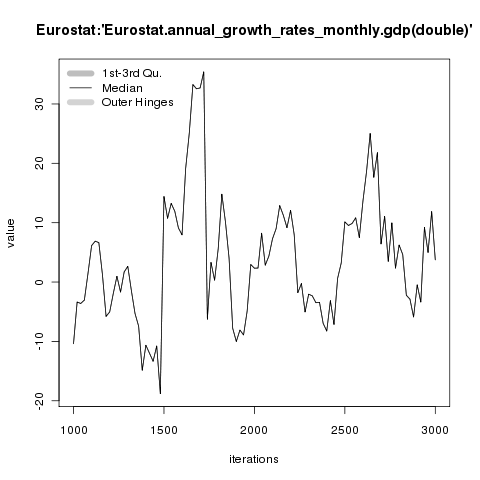
\includegraphics[width=8cm]{./stabilization/png/Eurostat-annual_growth_rates_monthly-gdp.png}
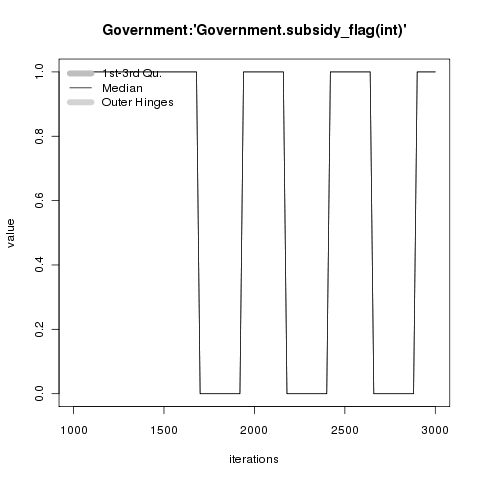
\includegraphics[width=8cm]{./stabilization/png/Government-subsidy_flag.png}
\end{minipage}
\caption{Effect of the stabilization policy in the energy shock experiment. Left panel: annual growth rate of GDP; right panel: activation of the subsidy regime by the government, which is lagged following the calendar year of $240 days$.}
\label{Figure: Stabilization}
\end{figure}
%\pagebreak 
